%%mark = star, diamond, square, otimes
%\documentclass{article}
%\usepackage{pgfplots}
%\usepackage[justification=centering]{caption}
%\pgfplotsset{compat=newest} 	title={\parbox{\linewidth}{\centering Total Tree Construction Time vs Minimum Suppport (\%) for T40I10D100K ~\cite{dataset}, Window Size = 5, Frame Size = 7000}},
%\begin{document}
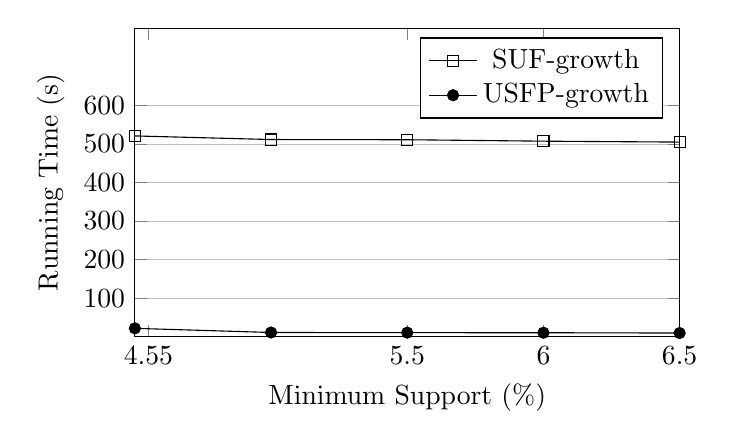
\begin{tikzpicture}
	\begin{axis}[
    width=8.5cm,
    height=5.5cm,
    xlabel={Minimum Support (\%) },
    ylabel={Running Time (s)},
    xmin=4.5, xmax=6.5,
    ymin=0, ymax=800,
    xtick={4.55,5.5,6,6.5},
    ytick={100,200,300,400,500,600},
    legend pos=north east,
    ymajorgrids=true,
    grid style={line width=.2pt,draw=gray!50},
]
 
\addplot[
    solid, every mark/.append style={solid, fill=gray}, mark=square
    ]
    coordinates {
			(4.5,520.723)
			(5  ,511.365)
			(5.5,510.854)
			(6  ,507.12 )
			(6.5,504.767)


	};
    \addlegendentry{SUF-growth}
\addplot[
    solid, every mark/.append style={solid, fill=black}, mark=*
    ]
    coordinates {
		(4.5,21.814)
		(5  ,11.035)
		(5.5,10.601)
		(6  ,10.423)
		(6.5,9.646 )


};
    \addlegendentry{USFP-growth}
 
\end{axis}
\end{tikzpicture}
%\end{document}